\documentclass[aspectratio=169,11pt]{beamer}

% =========================================================
% PACKAGES
% =========================================================
\usepackage{amsmath,amssymb,mathtools}
\usepackage{booktabs}
\usepackage{array}
\usepackage{tikz}
\usetikzlibrary{arrows.meta,positioning,calc}
\usepackage{pgfplots}
\pgfplotsset{compat=1.18}

% =========================================================
% THEME / CLEAN MINIMAL DESIGN
% =========================================================
\usetheme{default}

\definecolor{CUSATblue}{RGB}{25,65,115}
\definecolor{darkgray}{RGB}{55,55,55}
\definecolor{lightgray}{RGB}{235,238,242}

\setbeamercolor{normal text}{fg=darkgray,bg=white}
\setbeamercolor{structure}{fg=CUSATblue}
\setbeamercolor{frametitle}{fg=CUSATblue,bg=white}
\setbeamercolor{title}{fg=CUSATblue}
\setbeamercolor{subtitle}{fg=darkgray}

\setbeamertemplate{navigation symbols}{}

\setbeamertemplate{frametitle}{
    \vspace{0.35cm}
    \insertframetitle
    \vspace{0.15cm}
    \par\noindent
    {\color{CUSATblue}\rule{\textwidth}{0.7pt}}
}

\setbeamertemplate{footline}{
    \hfill
    \color{darkgray}\scriptsize\insertframenumber
    \hspace{0.4cm}\vspace{0.25cm}
}

\setbeamertemplate{itemize item}{\color{CUSATblue}\small$\bullet$}
\setbeamertemplate{itemize subitem}{\color{CUSATblue}\scriptsize$\bullet$}

% =========================================================
% COMMANDS
% =========================================================
\newcommand{\R}{\mathbb{R}}
\newcommand{\E}{\mathbb{E}}
\newcommand{\Var}{\operatorname{Var}}
\newcommand{\Cov}{\operatorname{Cov}}
\newcommand{\Bias}{\operatorname{Bias}}
\newcommand{\MSE}{\operatorname{MSE}}
\newcommand{\norm}[1]{\left\lVert #1\right\rVert}

% =========================================================
% TITLE
% =========================================================
\title{\textbf{Module 3: Statistics}}
\subtitle{Descriptive Statistics, Frequentist Statistics and Mathematical Foundations}
\author{Glenda Pinhero \\ M.Tech CSE  AI \& SE}
\institute{Cochin University of Science and Technology}
\date{Sept 2026}

\begin{document}

% =========================================================
% 1
% =========================================================
\begin{frame}
    \titlepage
\end{frame}

% =========================================================
% 2
% =========================================================
\begin{frame}{Module 3: Overview}

\begin{columns}[T]

\column{0.48\textwidth}
\textbf{Statistics}
\begin{itemize}
    \item Descriptive statistics
    \item Sampling
    \item Estimation
    \item MSE
    \item Confidence intervals
    \item Parametric and non-parametric estimation
\end{itemize}

\column{0.48\textwidth}
\textbf{Mathematical Foundations}
\begin{itemize}
    \item Algebraic structures
    \item Vector spaces
    \item Vectors
    \item Dot product
    \item Orthogonality
    \item Hyperplanes
\end{itemize}

\end{columns}
\end{frame}

% =========================================================
% SECTION 1
% =========================================================

% 3
\begin{frame}
\centering
\vfill
{\Huge\color{CUSATblue}\textbf{1. Introduction to Statistics}}
\vfill
\end{frame}

% 4
\begin{frame}{What is Statistics?}

\begin{block}{Definition}
Statistics is the science of collecting, organizing, summarizing,
analyzing and interpreting data.
\end{block}

\vspace{0.3cm}

\textbf{Two major branches}

\begin{itemize}
    \item \textbf{Descriptive statistics} -- summarizes observed data.
    \item \textbf{Inferential statistics} -- draws conclusions about a population from a sample.
\end{itemize}

\[
\boxed{\text{Data}\rightarrow\text{Analysis}\rightarrow\text{Inference}\rightarrow\text{Decision}}
\]

\end{frame}

% 5
\begin{frame}{Data, Information and Knowledge}

\begin{center}

\begin{tikzpicture}[node distance=2.2cm,>=Latex]
\node[draw=none] (d) {\Large\textbf{Data}};
\node[draw=none,right=of d] (i) {\Large\textbf{Information}};
\node[draw=none,right=of i] (k) {\Large\textbf{Knowledge}};

\draw[->,thick,CUSATblue] (d)--node[above]{processing}(i);
\draw[->,thick,CUSATblue] (i)--node[above]{interpretation}(k);
\end{tikzpicture}
\end{center}

\vspace{0.5cm}

\begin{itemize}
    \item \textbf{Data:} raw facts or observations.
    \item \textbf{Information:} processed data with meaning.
    \item \textbf{Knowledge:} understanding obtained from information and patterns.
\end{itemize}

\end{frame}

% 6
\begin{frame}{Types of Data}

\begin{columns}[T]

\column{0.48\textwidth}
\textbf{Qualitative}
\begin{itemize}
    \item Categorical
    \item Nominal
    \item Ordinal
\end{itemize}

Examples:
\[
\text{Color, Grade, Department}
\]

\column{0.48\textwidth}
\textbf{Quantitative}
\begin{itemize}
    \item Numerical
    \item Discrete
    \item Continuous
\end{itemize}

Examples:
\[
\text{Age, Height, Number of Students}
\]

\end{columns}
\end{frame}

% =========================================================
% DESCRIPTIVE STATISTICS
% =========================================================

% 7
\begin{frame}
\centering
\vfill
{\Huge\color{CUSATblue}\textbf{2. Descriptive Statistics}}
\vfill
\end{frame}

% 8
\begin{frame}{Descriptive Statistics}

Descriptive statistics summarizes the important characteristics of observed data.

\begin{itemize}
    \item Measures of central tendency
    \item Measures of dispersion
    \item Graphical summaries
    \item Distribution shape
    \item Outlier detection
\end{itemize}

\vspace{0.4cm}

\[
\boxed{\text{Center}+\text{Spread}+\text{Shape}}
\]

\end{frame}

% 9
\begin{frame}{Measures of Central Tendency}

\begin{center}
\Large
\[
\boxed{\text{Mean}\qquad\text{Median}\qquad\text{Mode}}
\]
\end{center}

\begin{itemize}
    \item \textbf{Mean:} arithmetic average.
    \item \textbf{Median:} middle value after sorting.
    \item \textbf{Mode:} most frequently occurring value.
\end{itemize}

\[
\bar{x}=\frac{1}{n}\sum_{i=1}^{n}x_i
\]

\end{frame}

% 10
\begin{frame}{Sample Mean}

For observations
\[
x_1,x_2,\ldots,x_n,
\]
the sample mean is

\[
\boxed{
\bar{x}=\frac{1}{n}\sum_{i=1}^{n}x_i
}
\]

\begin{example}
For $2,4,6,8,10$:

\[
\bar{x}
=
\frac{2+4+6+8+10}{5}
=
6
\]
\end{example}

\end{frame}

% 11
\begin{frame}{Median and Mode}

\textbf{Median}

\begin{itemize}
    \item Sort the observations.
    \item Odd number of observations: middle value.
    \item Even number: average of two middle values.
\end{itemize}

\textbf{Mode}

\begin{itemize}
    \item Most frequently occurring observation.
    \item More than one mode may exist.
\end{itemize}

\[
2,3,3,4,7,8,10
\]

\[
\text{Median}=4,\qquad\text{Mode}=3
\]

\end{frame}

% 12
\begin{frame}{Measures of Dispersion}

Dispersion measures how widely observations are spread.

\begin{center}
\[
\boxed{
\text{Range}\quad
\text{Variance}\quad
\text{Standard Deviation}\quad
\text{IQR}
}
\]
\end{center}

\[
\text{Range}=\max(x_i)-\min(x_i)
\]

\[
s^2=
\frac{1}{n-1}
\sum_{i=1}^{n}(x_i-\bar{x})^2
\]

\[
s=\sqrt{s^2}
\]

\end{frame}

% 13
\begin{frame}{Sample Variance}

\[
\boxed{
s^2=
\frac{1}{n-1}
\sum_{i=1}^{n}(x_i-\bar{x})^2
}
\]

\begin{itemize}
    \item Measures spread around the sample mean.
    \item Squaring prevents positive and negative deviations from cancelling.
    \item $n-1$ is used for the usual unbiased estimator of population variance.
\end{itemize}

Population variance:

\[
\sigma^2=
\frac{1}{N}
\sum_{i=1}^{N}(x_i-\mu)^2
\]

\end{frame}

% 14
\begin{frame}{Variance and Standard Deviation}

\[
\Var(X)=\E[X^2]-[\E(X)]^2
\]

\begin{itemize}
    \item Variance is measured in squared units.
    \item Standard deviation is measured in the original units.
    \item Higher variance indicates greater spread.
\end{itemize}

\[
\boxed{s=\sqrt{s^2}}
\]

\end{frame}

% 15
\begin{frame}{Histogram}

A histogram displays the frequency or density of numerical observations across intervals called \textbf{bins}.

\begin{center}
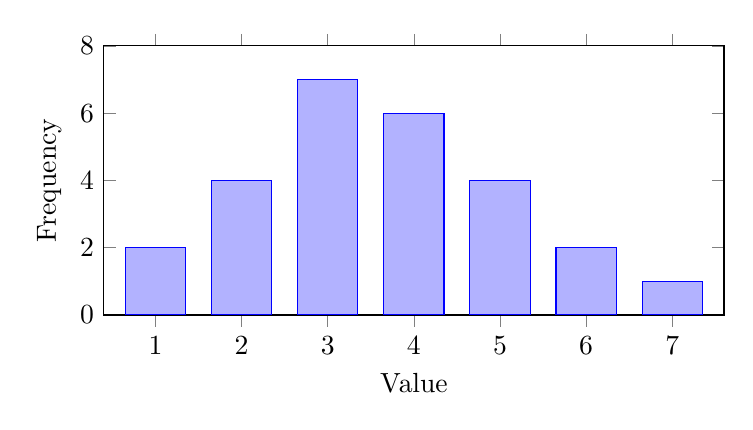
\begin{tikzpicture}
\begin{axis}[
    width=0.78\textwidth,
    height=5cm,
    xlabel={Value},
    ylabel={Frequency},
    ymin=0,
    ymax=8,
    xtick={1,2,3,4,5,6,7},
    ytick={0,2,4,6,8},
    ybar,
    bar width=0.7
]
\addplot coordinates {
(1,2) (2,4) (3,7) (4,6) (5,4) (6,2) (7,1)
};
\end{axis}
\end{tikzpicture}
\end{center}

\end{frame}

% 16
\begin{frame}{Reading a Histogram}

A histogram can reveal:

\begin{itemize}
    \item Center
    \item Spread
    \item Skewness
    \item Number of modes
    \item Possible unusual observations
\end{itemize}

\begin{alertblock}{Important}
The appearance of a histogram depends on the choice of bin width.
\end{alertblock}

\end{frame}

% 17
\begin{frame}{Boxplot}

A boxplot summarizes data using:

\[
\boxed{
\min,\quad Q_1,\quad
\text{Median},\quad Q_3,\quad\max
}
\]

\begin{center}
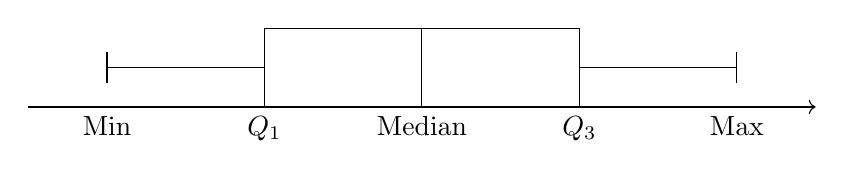
\begin{tikzpicture}
\draw[->] (0,0)--(10,0);

\draw (1,0.5)--(3,0.5);
\draw (7,0.5)--(9,0.5);

\draw (3,0) rectangle (7,1);
\draw (5,0)--(5,1);

\draw (1,0.3)--(1,0.7);
\draw (9,0.3)--(9,0.7);

\node[below] at (1,0){Min};
\node[below] at (3,0){$Q_1$};
\node[below] at (5,0){Median};
\node[below] at (7,0){$Q_3$};
\node[below] at (9,0){Max};
\end{tikzpicture}
\end{center}

\[
IQR=Q_3-Q_1
\]

\end{frame}

% 18
\begin{frame}{Outliers}

An \textbf{outlier} is an observation unusually far from the majority of observations.

Using the IQR rule:

\[
\boxed{
\text{Lower Fence}=Q_1-1.5IQR
}
\]

\[
\boxed{
\text{Upper Fence}=Q_3+1.5IQR
}
\]

Observations outside these limits are commonly flagged as outliers.

\end{frame}

% 19
\begin{frame}{Effect of Outliers}

Outliers can strongly influence:

\begin{itemize}
    \item Mean
    \item Variance
    \item Standard deviation
    \item Statistical models
\end{itemize}

More robust measures include:

\[
\boxed{\text{Median and IQR}}
\]

\begin{alertblock}{Key idea}
A single extreme observation can significantly change the mean, while the median may remain relatively stable.
\end{alertblock}

\end{frame}

% 20
\begin{frame}{Kurtosis}

Kurtosis describes the \textbf{tail heaviness} of a distribution.

\[
\boxed{
\beta_2=
\frac{\E[(X-\mu)^4]}{\sigma^4}
}
\]

\begin{itemize}
    \item \textbf{Mesokurtic:} normal-like reference.
    \item \textbf{Leptokurtic:} heavier tails.
    \item \textbf{Platykurtic:} lighter tails.
\end{itemize}

Excess kurtosis:

\[
\boxed{\gamma_2=\beta_2-3}
\]

\end{frame}

% =========================================================
% ORDER STATISTICS
% =========================================================

% 21
\begin{frame}{Order Statistics}

Given:
\[
X_1,X_2,\ldots,X_n
\]

sort the observations:

\[
X_{(1)}
\le
X_{(2)}
\le
\cdots
\le
X_{(n)}
\]

where $X_{(i)}$ is the $i$th order statistic.

\begin{itemize}
    \item $X_{(1)}$ = minimum
    \item $X_{(n)}$ = maximum
    \item Middle order statistics determine the median.
\end{itemize}

\end{frame}

% 22
\begin{frame}{Applications of Order Statistics}

Order statistics are used for:

\begin{itemize}
    \item Ranking
    \item Median calculation
    \item Quartiles
    \item Percentiles
    \item Boxplots
    \item Extreme-value analysis
\end{itemize}

Example:

\[
7,2,9,4,1
\]

\[
1,2,4,7,9
\]

Therefore:

\[
X_{(1)}=1,\qquad X_{(3)}=4,\qquad X_{(5)}=9.
\]

\end{frame}

% =========================================================
% COVARIANCE
% =========================================================

% 23
\begin{frame}
\centering
\vfill
{\Huge\color{CUSATblue}\textbf{3. Covariance}}
\vfill
\end{frame}

% 24
\begin{frame}{Sample Covariance}

For paired observations $(x_i,y_i)$:

\[
\boxed{
s_{xy}
=
\frac{1}{n-1}
\sum_{i=1}^{n}
(x_i-\bar{x})(y_i-\bar{y})
}
\]

Interpretation:

\begin{itemize}
    \item $s_{xy}>0$: variables tend to increase together.
    \item $s_{xy}<0$: one tends to increase as the other decreases.
    \item $s_{xy}\approx0$: little linear co-movement.
\end{itemize}

\end{frame}

% 25
\begin{frame}{Covariance and Variance}

Variance is a special case of covariance:

\[
\boxed{
\Cov(X,X)=\Var(X)
}
\]

\begin{center}
\begin{tabular}{lll}
\toprule
 & Variance & Covariance\\
\midrule
Variables & One & Two\\
Measures & Spread & Joint variation\\
Sign & Non-negative & +, $-$ or 0\\
\bottomrule
\end{tabular}
\end{center}

\end{frame}

% 26
\begin{frame}{Sample Covariance Matrix}

For

\[
\mathbf{X}
=
\begin{bmatrix}
X_1\\X_2\\\vdots\\X_p
\end{bmatrix},
\]

the covariance matrix is

\[
\boxed{
\Sigma=
\begin{bmatrix}
\Var(X_1)&\Cov(X_1,X_2)&\cdots\\
\Cov(X_2,X_1)&\Var(X_2)&\cdots\\
\vdots&\vdots&\ddots
\end{bmatrix}
}
\]

\begin{itemize}
    \item Diagonal = variances
    \item Off-diagonal = covariances
    \item Symmetric matrix
\end{itemize}

\end{frame}

% 27
\begin{frame}{Example: Covariance Matrix}

Suppose:

\[
\Var(X_1)=4,\qquad
\Var(X_2)=9,\qquad
\Cov(X_1,X_2)=3.
\]

Then:

\[
\boxed{
S=
\begin{bmatrix}
4&3\\
3&9
\end{bmatrix}
}
\]

The positive covariance indicates positive linear co-movement.

\end{frame}

% =========================================================
% ALGEBRA
% =========================================================

% 28
\begin{frame}
\centering
\vfill
{\Huge\color{CUSATblue}\textbf{4. Algebraic Structures}}
\vfill
\end{frame}

% 29
\begin{frame}{Algebraic Structures}

An algebraic structure consists of:

\begin{center}
\[
\boxed{\text{Set}+\text{Operation(s)}+\text{Axioms}}
\]
\end{center}

A binary operation:

\[
*:S\times S\rightarrow S
\]

Important properties:

\begin{itemize}
    \item Closure
    \item Associativity
    \item Identity
    \item Inverse
    \item Commutativity
\end{itemize}

\end{frame}

% 30
\begin{frame}{Semigroup and Monoid}

\textbf{Semigroup}

A set with a closed and associative binary operation:

\[
(a*b)*c=a*(b*c)
\]

\textbf{Monoid}

A semigroup with an identity element $e$:

\[
e*a=a*e=a
\]

\[
\boxed{
\text{Monoid}
=
\text{Semigroup}
+
\text{Identity}
}
\]

\end{frame}

% 31
\begin{frame}{Group}

A group $(G,*)$ satisfies:

\begin{enumerate}
    \item Closure
    \item Associativity
    \item Identity
    \item Inverse
\end{enumerate}

For every $a\in G$:

\[
\exists a^{-1}\in G
\]

such that

\[
aa^{-1}=a^{-1}a=e.
\]

Example:

\[
(\mathbb Z,+)
\]

\end{frame}

% 32
\begin{frame}{Abelian Group}

An Abelian group is a group that is also commutative.

\[
\boxed{
a*b=b*a
}
\]

for all $a,b\in G$.

Example:

\[
(\mathbb Z,+)
\]

because:

\[
a+b=b+a.
\]

\begin{alertblock}{Key point}
Every Abelian group is a group, but every group need not be Abelian.
\end{alertblock}

\end{frame}

% 33
\begin{frame}{Ring}

A ring has two operations:

\[
+,\qquad\times
\]

Typically:

\[
(R,+)
\]

is an Abelian group, while multiplication is associative and distributive over addition.

\[
a(b+c)=ab+ac
\]

\[
(a+b)c=ac+bc
\]

Example:

\[
\boxed{\mathbb Z}
\]

is a ring.

\end{frame}

% 34
\begin{frame}{Field}

A field is a commutative ring in which every non-zero element has a multiplicative inverse.

For $a\neq0$:

\[
\exists a^{-1}
\]

such that

\[
aa^{-1}=1.
\]

Examples:

\[
\boxed{
\mathbb Q,\quad\mathbb R,\quad\mathbb C
}
\]

\end{frame}

% 35
\begin{frame}{Algebraic Structure Hierarchy}

\begin{center}

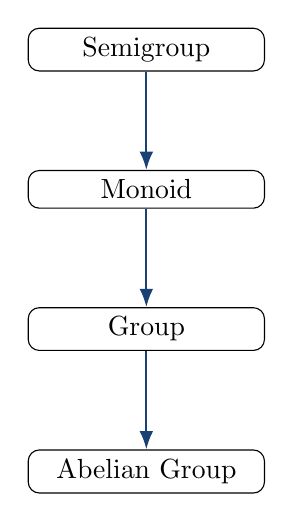
\begin{tikzpicture}[node distance=1.25cm,>=Latex]

\node[draw,rounded corners,minimum width=3cm] (s) {Semigroup};
\node[draw,rounded corners,minimum width=3cm,below=of s] (m) {Monoid};
\node[draw,rounded corners,minimum width=3cm,below=of m] (g) {Group};
\node[draw,rounded corners,minimum width=3cm,below=of g] (a) {Abelian Group};

\draw[->,thick,CUSATblue] (s)--(m);
\draw[->,thick,CUSATblue] (m)--(g);
\draw[->,thick,CUSATblue] (g)--(a);

\end{tikzpicture}

\hspace{1.5cm}

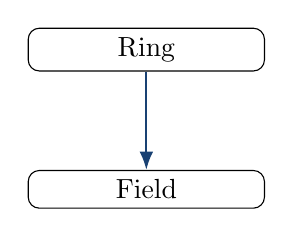
\begin{tikzpicture}[node distance=1.25cm,>=Latex]
\node[draw,rounded corners,minimum width=3cm] (r) {Ring};
\node[draw,rounded corners,minimum width=3cm,below=of r] (f) {Field};
\draw[->,thick,CUSATblue] (r)--(f);
\end{tikzpicture}

\end{center}

\end{frame}

% =========================================================
% VECTOR SPACES
% =========================================================

% 36
\begin{frame}
\centering
\vfill
{\Huge\color{CUSATblue}\textbf{5. Vector Spaces and Vectors}}
\vfill
\end{frame}

% 37
\begin{frame}{Mathematical Spaces}

A mathematical space is a set of objects together with structure that allows relationships between them to be studied.

Examples:

\begin{itemize}
    \item Metric spaces -- distance
    \item Topological spaces -- continuity and neighborhoods
    \item Vector spaces -- vector operations
    \item Probability spaces -- outcomes and probabilities
\end{itemize}

\end{frame}

% 38
\begin{frame}{Vector Space}

A vector space $V$ over a field $F$ supports:

\begin{itemize}
    \item Vector addition
    \item Scalar multiplication
\end{itemize}

For $\mathbf u,\mathbf v\in V$ and $a,b\in F$:

\[
\boxed{
a\mathbf u+b\mathbf v\in V
}
\]

Important properties include:

\begin{itemize}
    \item Additive identity $\mathbf0$
    \item Additive inverse $-\mathbf v$
    \item Associativity and commutativity of addition
    \item Distributivity of scalar multiplication
\end{itemize}

\end{frame}

% 39
\begin{frame}{What is a Vector?}

A vector has:

\[
\boxed{\text{Magnitude + Direction}}
\]

A vector in $\R^n$ can be written as:

\[
\mathbf v=
\begin{bmatrix}
v_1\\v_2\\\vdots\\v_n
\end{bmatrix}
\]

Its Euclidean magnitude is:

\[
\boxed{
\norm{\mathbf v}
=
\sqrt{v_1^2+\cdots+v_n^2}
}
\]

\end{frame}

% 40
\begin{frame}{Scalar Multiplication}

For a scalar $c$:

\[
\boxed{
\mathbf v'=c\mathbf v
}
\]

Magnitude:

\[
\boxed{
\norm{c\mathbf v}
=
|c|\norm{\mathbf v}
}
\]

\begin{itemize}
    \item $|c|>1$: magnitude increases.
    \item $0<|c|<1$: magnitude decreases.
    \item $c=0$: zero vector.
    \item $c<0$: direction reverses.
\end{itemize}

\end{frame}

% 41
\begin{frame}{Changing the Magnitude of a Vector}

Let

\[
\mathbf v=(2,1).
\]

Then:

\[
2\mathbf v=(4,2)
\]

has twice the magnitude.

\[
\frac12\mathbf v=
\left(1,\frac12\right)
\]

has half the magnitude.

\[
-\mathbf v=(-2,-1)
\]

has the same magnitude but opposite direction.

\end{frame}

% 42
\begin{frame}{Vector Addition}

For

\[
\mathbf u=
\begin{bmatrix}
u_1\\u_2
\end{bmatrix},
\qquad
\mathbf v=
\begin{bmatrix}
v_1\\v_2
\end{bmatrix},
\]

\[
\boxed{
\mathbf u+\mathbf v
=
\begin{bmatrix}
u_1+v_1\\
u_2+v_2
\end{bmatrix}
}
\]

Vector addition is component-wise.

\end{frame}

% 43
\begin{frame}{Impact of Vector Addition}

The resultant depends on the angle between the vectors.

\textbf{Same direction}

\[
\norm{\mathbf u+\mathbf v}
=
\norm{\mathbf u}+\norm{\mathbf v}
\]

\textbf{Opposite directions}

Vectors can partially or completely cancel.

\textbf{Perpendicular vectors}

\[
\norm{\mathbf u+\mathbf v}
=
\sqrt{
\norm{\mathbf u}^2+
\norm{\mathbf v}^2
}
\]

\end{frame}

% 44
\begin{frame}{Dot Product}

For $\mathbf u,\mathbf v\in\R^n$:

\[
\boxed{
\mathbf u\cdot\mathbf v
=
\sum_{i=1}^{n}u_iv_i
}
\]

Geometrically:

\[
\boxed{
\mathbf u\cdot\mathbf v
=
\norm{\mathbf u}
\norm{\mathbf v}
\cos\theta
}
\]

where $\theta$ is the angle between the vectors.

\end{frame}

% 45
\begin{frame}{Orthogonal Vectors}

Two non-zero vectors are orthogonal if:

\[
\theta=90^\circ.
\]

Using:

\[
\mathbf u\cdot\mathbf v
=
\norm{\mathbf u}
\norm{\mathbf v}
\cos\theta,
\]

we get:

\[
\mathbf u\cdot\mathbf v
=
\norm{\mathbf u}
\norm{\mathbf v}
\cos90^\circ
\]

Therefore:

\[
\boxed{
\mathbf u\cdot\mathbf v=0
}
\]

\end{frame}

% 46
\begin{frame}{Proof of Orthogonality}

Suppose:

\[
\mathbf u\perp\mathbf v.
\]

Then:

\[
\theta=90^\circ.
\]

By the dot-product formula:

\[
\mathbf u\cdot\mathbf v
=
\norm{\mathbf u}
\norm{\mathbf v}
\cos\theta.
\]

Substitute $\theta=90^\circ$:

\[
\mathbf u\cdot\mathbf v
=
\norm{\mathbf u}
\norm{\mathbf v}(0)
\]

Hence: $\boxed{
\mathbf u\cdot\mathbf v=0
}$

\end{frame}

% 47
\begin{frame}{Two Aligned Unit Vectors}

Let $\mathbf u$ and $\mathbf v$ be unit vectors:

\[
\norm{\mathbf u}
=
\norm{\mathbf v}
=
1.
\]

If they are aligned:

\[
\theta=0^\circ.
\]

Therefore:

\[
\mathbf u\cdot\mathbf v
=
(1)(1)\cos0^\circ
\]

\[
\boxed{
\mathbf u\cdot\mathbf v=1
}
\]

\end{frame}

% =========================================================
% HYPERPLANE
% =========================================================

% 48
\begin{frame}{Hyperplane}

A hyperplane in $\R^n$ can be represented by:

\[
\boxed{
\mathbf w^T\mathbf x+b=0
}
\]

where:

\begin{itemize}
    \item $\mathbf w$ = normal vector
    \item $\mathbf x$ = point
    \item $b$ = bias/intercept
\end{itemize}

Examples:

\[
\R^2:\text{ line}
\]

\[
\R^3:\text{ plane}
\]

\[
\R^n:\text{ $(n-1)$-dimensional hyperplane}
\]

\end{frame}

% 49
\begin{frame}{Changing the Orientation of a Hyperplane}

The vector $\mathbf w$ is normal to the hyperplane:

\[
\mathbf w^T\mathbf x+b=0.
\]

Changing the direction of $\mathbf w$ changes the orientation of the normal and therefore the orientation of the hyperplane.

For a linear classifier:

\[
\boxed{
f(\mathbf x)=\mathbf w^T\mathbf x+b
}
\]

the hyperplane:

\[
f(\mathbf x)=0
\]

acts as the decision boundary.

\end{frame}

% 50
\begin{frame}{Vectors and Hyperplanes in Machine Learning}

A feature vector:

\[
\mathbf x=
\begin{bmatrix}
x_1\\x_2\\\vdots\\x_n
\end{bmatrix}
\]

is classified using:

\[
\mathbf w^T\mathbf x+b.
\]

\begin{itemize}
    \item $\mathbf x$ -- feature vector
    \item $\mathbf w$ -- weight vector
    \item $b$ -- bias
    \item $\mathbf w$ -- normal to decision boundary
\end{itemize}
\boxed{
\text{Linear classifier}
\longleftrightarrow
\text{Hyperplane}
}

\end{frame}

% =========================================================
% FREQUENTIST
% =========================================================

% 51
\begin{frame}
\centering
\vfill
{\Huge\color{CUSATblue}\textbf{6. Frequentist Statistics}}
\vfill
\end{frame}

% 52
\begin{frame}{Frequentist Statistics}

Frequentist statistics interprets probability through the behavior of repeated random sampling.

\begin{center}
\[
\boxed{
\text{Population}
\rightarrow
\text{Sample}
\rightarrow
\text{Statistic}
\rightarrow
\text{Inference}
}
\]
\end{center}

\textbf{Parameter}

\[
\mu,\sigma^2
\]

Fixed but generally unknown.

\textbf{Statistic}

\[
\bar X,S^2
\]

Calculated from a sample.

\end{frame}

% 53
\begin{frame}{Sampling}

\textbf{Population}

Complete collection of units or observations of interest.

\textbf{Sample}

Subset selected from the population.

Common approaches:

\begin{itemize}
    \item Simple random sampling
    \item Stratified sampling
    \item Systematic sampling
    \item Cluster sampling
\end{itemize}

\end{frame}

% 54
\begin{frame}{Sampling Distribution}

A sampling distribution is the probability distribution of a statistic over repeated samples.

For the sample mean:

\[
\E[\bar X]=\mu
\]

and, under independent sampling,

\[
\boxed{
\Var(\bar X)=\frac{\sigma^2}{n}
}
\]

As $n$ increases, the sampling variability of $\bar X$ decreases.

\end{frame}

% 55
\begin{frame}{Point Estimation}

An \textbf{estimator} is a rule for estimating an unknown population parameter.

Example:

\[
\boxed{
\hat\mu=\bar X
}
\]

estimates $\mu$.

\textbf{Estimator vs Estimate}

\begin{itemize}
    \item Estimator -- rule/random quantity.
    \item Estimate -- numerical value obtained after observing data.
\end{itemize}

\end{frame}

% 56
\begin{frame}{Mean Square Error}

For an estimator $\hat\theta$:

\[
\boxed{
\MSE(\hat\theta)
=
\E[(\hat\theta-\theta)^2]
}
\]

MSE measures expected squared estimation error.

It incorporates:

\[
\boxed{
\text{Variance}+\text{Squared Bias}
}
\]

\end{frame}

% 57
\begin{frame}{Bias--Variance Decomposition}

Bias:

\[
\boxed{
\Bias(\hat\theta)
=
\E[\hat\theta]-\theta
}
\]

MSE decomposition:

\[
\boxed{
\MSE(\hat\theta)
=
\Var(\hat\theta)
+
\Bias(\hat\theta)^2
}
\]

Thus, a good estimator should balance bias and variability.

\end{frame}

% 58
\begin{frame}{Consistency and Confidence Intervals}

\textbf{Consistency}

An estimator is consistent if it approaches the true parameter as sample size increases:

\[
\boxed{
\hat\theta_n\xrightarrow{P}\theta
}
\]

\textbf{Confidence interval}

General form:

\[
\boxed{
\text{Estimate}
\pm
\text{Critical value}
\times
\text{Standard Error}
}
\]

\end{frame}

% 59
\begin{frame}{Parametric and Non-Parametric Estimation}

\begin{center}
\begin{tabular}{p{0.36\textwidth}p{0.27\textwidth}p{0.27\textwidth}}
\toprule
\textbf{Feature} & \textbf{Parametric} & \textbf{Non-parametric}\\
\midrule
Assumptions & Stronger & Fewer\\
Parameters & Fixed/finite & Flexible\\
Flexibility & Lower & Higher\\
Example & Normal model & KDE\\
\bottomrule
\end{tabular}
\end{center}

\vspace{0.3cm}

Parametric models are efficient when assumptions are appropriate.

Non-parametric methods are more flexible but may require more data.

\end{frame}

% =========================================================
% FORMULA SUMMARY
% =========================================================

% 60
\begin{frame}{Module 3 -- Formula Summary}

\small

\begin{align*}
\text{Mean:}\quad&
\bar{x}=\frac1n\sum_{i=1}^{n}x_i
\\[4pt]
\text{Variance:}\quad&
s^2=\frac1{n-1}\sum_{i=1}^{n}(x_i-\bar{x})^2
\\[4pt]
\text{IQR:}\quad&
IQR=Q_3-Q_1
\\[4pt]
\text{Covariance:}\quad&
s_{xy}=
\frac1{n-1}\sum_{i=1}^{n}
(x_i-\bar{x})(y_i-\bar{y})
\\[4pt]
\text{Dot product:}\quad&
\mathbf u\cdot\mathbf v
=
\norm{\mathbf u}\norm{\mathbf v}\cos\theta
\\[4pt]
\text{Orthogonality:}\quad&
\mathbf u\cdot\mathbf v=0
\\[4pt]
\text{Vector scaling:}\quad&
\norm{c\mathbf v}=|c|\norm{\mathbf v}
\\[4pt]
\text{Hyperplane:}\quad&
\mathbf w^T\mathbf x+b=0
\\[4pt]
\text{MSE:}\quad&
\MSE(\hat\theta)
=
\Var(\hat\theta)+\Bias(\hat\theta)^2
\end{align*}

\end{frame}

\end{document}